\begin{figure}[htbp]
\centering
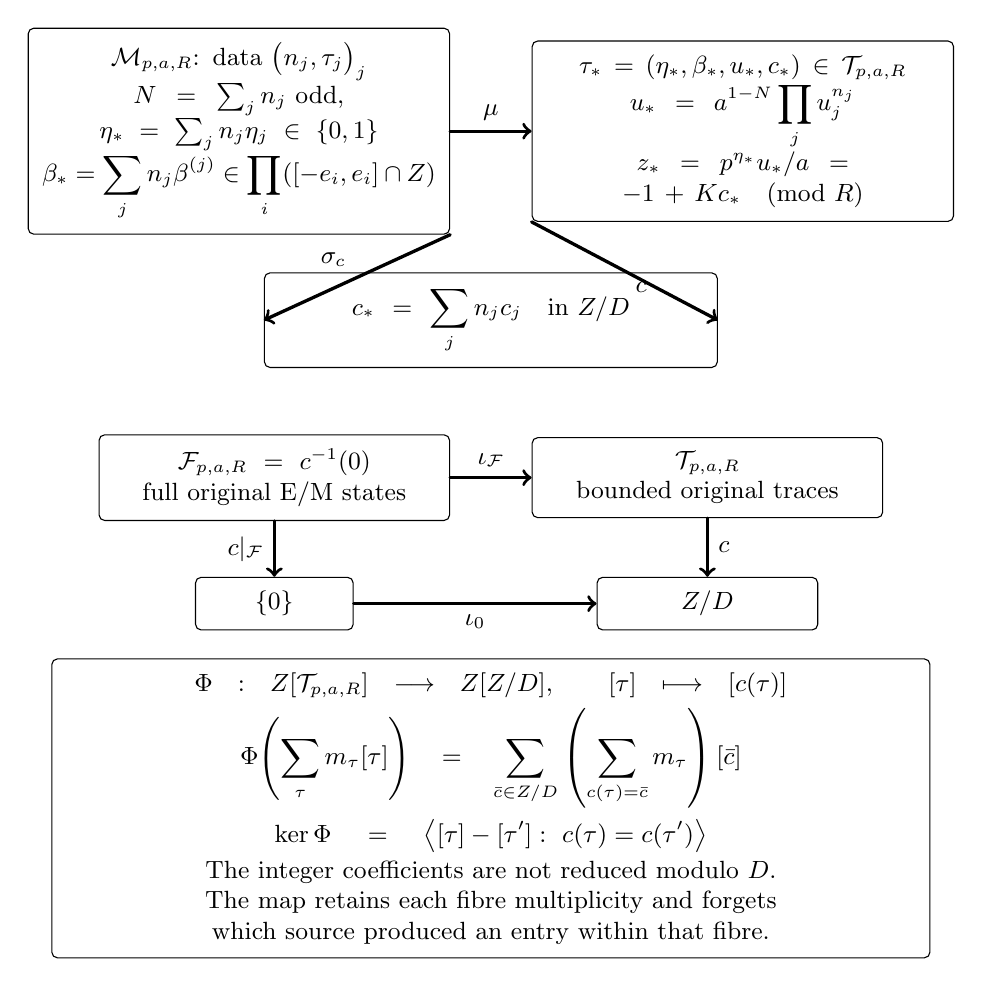
\begin{tikzpicture}[
  font=\small,
  box/.style={draw,rounded corners=2pt,align=center,inner sep=5pt},
  every path/.style={line cap=round,line join=round}
]
  \node[box,text width=5.0cm] (mix) at (-3.2,4.35)
    {$\mathcal M_{p,a,R}$: data $\bigl(n_j,\tau_j\bigr)_j$\\
     $N=\sum_j n_j$ odd,\quad
     $\eta_*=\sum_jn_j\eta_j\in\{0,1\}$\\
     $\displaystyle
       \beta_*=\sum_jn_j\beta^{(j)}
       \in\prod_i([-e_i,e_i]\cap\mathbb Z)$};
  \node[box,text width=5.0cm] (trace-star) at (3.2,4.35)
    {$\tau_*=(\eta_*,\beta_*,u_*,c_*)
       \in\mathcal T_{p,a,R}$\\
     $\displaystyle u_*=a^{1-N}\prod_j u_j^{n_j}$\\
     $z_*=p^{\eta_*}u_*/a=-1+Kc_*\pmod R$};
  \node[box,text width=5.4cm] (defect-sum) at (0,1.95)
    {$\displaystyle c_*=\sum_jn_jc_j\quad\hbox{in }\mathbb Z/D$};

  \draw[->,very thick] (mix) -- node[above]
    {$\mu$} (trace-star);
  \draw[->,very thick] (mix.south east) -- node[above left]
    {$\sigma_c$} (defect-sum.west);
  \draw[->,very thick] (trace-star.south west) -- node[below right]
    {$c$} (defect-sum.east);

  \node[box,text width=4.1cm] (full) at (-2.75,-0.05)
    {$\mathcal F_{p,a,R}=c^{-1}(0)$\\
     full original E/M states};
  \node[box,text width=4.1cm] (traces-fibre) at (2.75,-0.05)
    {$\mathcal T_{p,a,R}$\\bounded original traces};
  \node[box,text width=1.65cm] (zero) at (-2.75,-1.65)
    {$\{0\}$};
  \node[box,text width=2.45cm] (defect-fibre) at (2.75,-1.65)
    {$\mathbb Z/D$};
  \draw[->,very thick] (full) -- node[above]
    {$\iota_{\mathcal F}$} (traces-fibre);
  \draw[->,very thick] (full) -- node[left]
    {$c|_{\mathcal F}$} (zero);
  \draw[->,very thick] (traces-fibre) -- node[right]
    {$c$} (defect-fibre);
  \draw[->,very thick] (zero) -- node[below]
    {$\iota_0$} (defect-fibre);

  \node[box,text width=10.8cm] (module) at (0,-4.25)
    {$\displaystyle
      \Phi:\mathbb Z[\mathcal T_{p,a,R}]
      \longrightarrow\mathbb Z[\mathbb Z/D],\qquad
      [\tau]\longmapsto[c(\tau)]$\\[3pt]
     $\displaystyle
      \Phi\!\left(\sum_{\tau}m_\tau[\tau]\right)
      =\sum_{\bar c\in\mathbb Z/D}
       \left(\sum_{c(\tau)=\bar c}m_\tau\right)[\bar c]$\\[3pt]
     $\displaystyle
      \ker\Phi=
      \left\langle[\tau]-[\tau']:\ c(\tau)=c(\tau')\right\rangle$\\[2pt]
     The integer coefficients are not reduced modulo $D$.
     The map retains each fibre multiplicity and forgets which source produced
     an entry within that fibre.};
\end{tikzpicture}
\caption{Typed maps for the defect equation
$p^\eta u/a=-1+Kc\pmod R$.  In the upper triangle,
$\sigma_c((n_j,\tau_j)_j)=\sum_jn_jc_j$, and the triangle commutes by the
mixed integer-exponent law.  The middle square identifies the
full states as the zero fibre.  The lower map states the exact kernel and the
information lost when original trace words are replaced by their defect-bin
coefficient vector.}
\label{fig:defect-map}
\end{figure}
